\documentclass[modern]{aastex61}

% All the packages
%\usepackage[letterpaper]{geometry}
\usepackage{fontspec}
\usepackage{microtype}
\usepackage{url}
\usepackage{amsmath}
\usepackage{mathtools}
\usepackage{esint}
\usepackage{amssymb}
\usepackage{natbib}
\usepackage{multirow}
\usepackage{graphicx}
\usepackage{scalerel}
\usepackage{calc}
\usepackage{etoolbox}
\usepackage{marginnote}
\usepackage{nicefrac}
\usepackage{tabstackengine}
\usepackage{diagbox}
\usepackage[makeroom]{cancel}
\usepackage{mathdots}
\usepackage{bbm}
\usepackage{booktabs}
\usepackage{xspace}
\usepackage{upgreek}
\usepackage[T1]{fontenc} % https://tex.stackexchange.com/a/166791
\usepackage{textcomp}
\usepackage{ifxetex}
\ifxetex
\usepackage{fontspec}
\defaultfontfeatures{Extension = .otf}
\fi
\usepackage{fontawesome}
\usepackage{listings}
\usepackage{mathtools}
\stackMath

% Page breaks in long equations
%\allowdisplaybreaks

% Bibliography stuff
\bibliographystyle{aasjournal}

% Shorthand for this paper
\newcommand{\starry}{\textsf{starry}\xspace}
\newcommand{\batman}{\textsf{batman}\xspace}
\newcommand{\planetplanet}{\textsf{planetplanet}\xspace}
\newcommand{\Python}{\textsf{Python}\xspace}
\newcommand{\cpp}{\textsf{C}++\xspace}
\newcommand{\Mathematica}{\textsf{Mathematica}\xspace}

% editing
\newcommand{\todo}[1]{{\color{red}\textbf{TODO:} #1}}


% References to text content
\newcommand{\documentname}{\textsl{article}}
\newcommand{\figureref}[1]{\ref{fig:#1}}
\newcommand{\Figure}[1]{Figure~\figureref{#1}}
\newcommand{\figurelabel}[1]{\label{fig:#1}}
\renewcommand{\eqref}[1]{\ref{eq:#1}}
\newcommand{\Eq}[1]{Equation~(\eqref{#1})}
\newcommand{\eq}[1]{\Eq{#1}}
\newcommand{\eqalt}[1]{Equation~\eqref{#1}}
\newcommand{\eqlabel}[1]{\label{eq:#1}}

% Add code, proof, and animation hyperlinks
\definecolor{linkcolor}{rgb}{0.1216,0.4667,0.7059}
\newcommand{\codeicon}{{\color{linkcolor}\faFileCodeO}}
\newcommand{\prooficon}{{\color{linkcolor}\faPencilSquareO}}
\newcommand{\animicon}{{\color{linkcolor}\faPlayCircle}}
\input{gitlinks}

\newtagform{eqtag}[]{(}{)}
\newcommand{\currentlabel}{None}

% Define a proof environment
\newenvironment{proof}[1]{%
\ifstrempty{#1}{%
\renewtagform{eqtag}[]{\raisebox{-0.1em}{{\color{red}\faPencilSquareO}}\,(}{)}%
}{%
\renewtagform{eqtag}[]{\prooflink{#1}\,(}{)}%
}%
\usetagform{eqtag}%
\renewcommand{\currentlabel}{#1}
\align%
}{%
\endalign%
\renewtagform{eqtag}[]{(}{)}%
\usetagform{eqtag}%
\message{<<<\currentlabel: \theequation>>>}%
}

% Define a proof environment
\newenvironment{proof*}[1]{%
\ifstrempty{#1}{%
\renewtagform{eqtag}[]{\raisebox{-0.1em}{{\color{red}\faPencilSquareO}}\,(}{)}%
}{%
\renewtagform{eqtag}[]{\prooflink{#1}\,(}{)}%
}%
\usetagform{eqtag}%
\renewcommand{\currentlabel}{#1}
\equation%
}{%
\endequation%
\renewtagform{eqtag}[]{(}{)}%
\usetagform{eqtag}%
\message{<<<\currentlabel: \theequation>>>}
}

% Math stuff
%\newcommand{\ii}{\ensuremath{\mathbf{i}}}
\newcommand{\T}{\ensuremath{\mathrm{T}}}
\newcommand{\dd}{\ensuremath{ \mathrm{d}}}
\newcommand{\unit}[1]{{\ensuremath{\mathrm{#1}}}}
\newcommand{\bvec}[1]{{\ensuremath{\mathbf{#1}}}}
\newcommand{\avec}[1]{{\ensuremath{\vec{\mathbf{#1}}}}}
\newcommand{\x}{\ensuremath{\mbox{$x$}}}
\newcommand{\y}{\ensuremath{\mbox{$y$}}}
\newcommand{\z}{\ensuremath{\mbox{$z$}}}
\newcommand{\xhat}{\ensuremath{\mathbf{\hat{x}}}}
\newcommand{\yhat}{\ensuremath{\mathbf{\hat{y}}}}
\newcommand{\zhat}{\ensuremath{\mathbf{\hat{z}}}}
\DeclareMathAlphabet\mathbfcal{OMS}{cmsy}{b}{n}
\DeclareMathOperator{\Tr}{Tr}
\DeclarePairedDelimiter\ceil{\lceil}{\rceil}
\DeclarePairedDelimiter\floor{\lfloor}{\rfloor}
\definecolor{dim}{rgb}{0.8,0.8,0.8}
\newcolumntype{L}[1]{>{\raggedright\let\newline\\\arraybackslash\hspace{0pt}}m{#1}}
\setcounter{MaxMatrixCols}{20}
\newcommand{\sinphi}{\ensuremath{\mbox{$u$}}}
\newcommand{\sinlambda}{\ensuremath{\mbox{$v$}}}
\newcommand{\bigdot}{\scaleto{\cdot}{6pt}}

% Bases
\newcommand{\ubasis}{\ensuremath{\tilde{\mathbf{u}}}}
\newcommand{\ubasisn}{\ensuremath{\tilde{\mathbf{u}}_n}}
\newcommand{\pbasis}{\ensuremath{\tilde{\mathfrak{p}}}}
\newcommand{\pbasisn}{\ensuremath{\tilde{\mathfrak{p}}_n}}
\newcommand{\gbasis}{\ensuremath{\tilde{\mathfrak{g}}}}
\newcommand{\gbasisn}{\ensuremath{\tilde{\mathfrak{g}}_n}}

% Code examples
\usepackage{listings}
\definecolor{codegreen}{rgb}{0,0.6,0}
\definecolor{codegray}{rgb}{0.5,0.5,0.5}
\definecolor{codepurple}{rgb}{0.58,0,0.82}
\definecolor{backcolour}{rgb}{0.95,0.95,0.95}
\lstdefinestyle{mystyle}{
    backgroundcolor=\color{backcolour},
    commentstyle=\color{codegreen},
    keywordstyle=\color{magenta},
    numberstyle=\tiny\color{codegray},
    stringstyle=\color{codepurple},
    basicstyle=\small\ttfamily,
    breakatwhitespace=false,
    breaklines=true,
    captionpos=b,
    keepspaces=true,
    numbers=left,
    numbersep=5pt,
    showspaces=false,
    showstringspaces=false,
    showtabs=false,
    tabsize=2,
    aboveskip=1em,
    belowskip=1em,
    keywords=[2]{map},
    keywordstyle=[2]{\color{black!80!black}},
}
\lstset{style=mystyle}

% Inverse diagonal dots
\makeatletter
\def\Ddots{\mathinner{\mkern1mu\raise\p@
\vbox{\kern7\p@\hbox{.}}\mkern2mu
\raise4\p@\hbox{.}\mkern2mu\raise7\p@\hbox{.}\mkern1mu}}
\makeatother

% Typography obsessions
\setlength{\parindent}{3.0ex}
\renewcommand\quad{\hskip\fontdimen3\font}

\usepackage{graphicx}

\begin{document}%\raggedbottom\sloppy\sloppypar\frenchspacing

\setlength{\abovedisplayskip}{1.5em}
\setlength{\belowdisplayskip}{1.5em}

\title{%
    Analytic Transit Light Curves for Limb-Darkened Stars
}

\author[0000-0002-0296-3826]{Rodrigo Luger}
\affil{Department~of~Astronomy, University~of~Washington, Seattle, WA}
\author{Eric Agol}
\affil{Department~of~Astronomy, University~of~Washington, Seattle, WA}

\keywords{methods: analytic --- techniques: photometric}

\begin{abstract}
    We derive analytic, closed-form solutions for the light curve
    of a planet transiting a star with a limb darkening profile of
    arbitrary integer order.  We provide updated expressions for the linear
    and quadratically limb darkened cases that are numerically stable
    over the entire domain.  Our expressions are fast to evaluate,
    allow for the integration over exposure time adaptively, and
    can be used to compute the first partial derivatives.
\end{abstract}

% ==============================================================================
% ------------------------------------------------------------------------------
% ------------------------------------------------------------------------------
%
\section{Introduction}
\label{sec:intro}
% ------------------------------------------------------------------------------
% ------------------------------------------------------------------------------
% ==============================================================================

\citet{Gimenez2006} derived transit light curves for a limb-darkening
function
\begin{equation}
I(\upmu) = I(1) \left[\sum_{n=1}^N u_n (1-\upmu^n) \right],
\end{equation}
where $\upmu = \cos{\theta} =\sqrt{1-r^2}$, where $\theta$ is the polar angle measured from the
sub-observer point), $r$ is the normalized stellar radius projected on the sky
$0\le r \le 1$, and $u_n$ is a limb-darkening coefficient.  \cite{Gimenez2006}
found an infinite series for computing the limb-darkened light curve for each $u_n$
term.  Here we present closed-form expressions for these terms which can be
easily computed with recursion relations.


\begin{itemize}
\item \cite{Pal2008} derived the partial derivatives of the quadratic limb-darkening model
with respect to $b$ and $r$.
\end{itemize}

% ==============================================================================
% ------------------------------------------------------------------------------
% ------------------------------------------------------------------------------
%
\section{Linear Limb-Darkening}
\label{sec:reparam}
% ------------------------------------------------------------------------------
% ------------------------------------------------------------------------------
% ==============================================================================

From \citet{MandelAgol2002}, the total flux visible during the occultation of a
body whose surface map is given by $I(x, y) = \sqrt{1 - \x^2 -\y^2}$ may be computed
as
%
\begin{align}
    \label{eq:s2}
    s_2 = \frac{2\pi}{3} \left(1 - \frac{3\Lambda(b,r)}{2} - \Theta(r - b) \right)
\end{align}
%
where $\Theta(\bigdot)$ is the Heaviside step function and
%
\begingroup\makeatletter\def\f@size{10}\check@mathfonts
\def\maketag@@@#1{\hbox{\m@th\large\normalfont#1}}%
\begin{align}
    \label{eq:biglam}
    \Lambda(b,r) &=
    \begin{dcases}
          % I don't think we need this: the k^2>1 term is stable as b --> 0!
          %-\frac{2}{3}\left(1 - r^2\right)^\frac{3}{2}
          %& \qquad b = 0
          %
          %\\[1.5em]
          %
          \frac{1}{9 \pi \sqrt{b r}} \Bigg[
                \frac{(r + b)^2 - 1}{r + b}
                \Big(
                    -2r \,
                    \big(
                        2 (r + b)^2 + (r + b)(r - b) - 3
                    \big)
                    K(k^2)
                    &\\ \phantom{XXXX}
                    + 3 (b - r) \, \Pi\big(k^2 (b + r)^2, \, k^2\big)
                \Big)
                - 4 b r (4 - 7 r^2 - b^2) E(k^2)
          \Bigg]
          %
          & \qquad k^2 < 1
          %
          \\[1.5em]
          %
          \frac{2}{9 \pi} \Bigg[
                \big(1 - (r + b)^2\big)
                \Bigg(
                    \sqrt{1 - (b - r)^2} \,
                    K\left(\frac{1}{k^2}\right)
                    + 3 \left(\frac{b-r}{(b+r)\sqrt{1 - (b - r)^2}}\right)
                    &\\ \phantom{XX}
                    \times \Pi\left(\frac{1}{k^2(b+r)^2}, \, \frac{1}{k^2}\right)
                \Bigg)
                - \sqrt{1 - (b - r)^2}
                (4 - 7 r^2 - b^2)
                E\left(\frac{1}{k^2}\right)
          \Bigg]
          %
          & \qquad k^2 \ge 1
    \end{dcases}
\end{align}
\endgroup
%
with
%
\begin{align}
    \label{eq:k2}
    k^2 &= \frac{1 - r^2 - b^2 + 2 b r}{4 b r}
    \quad.
\end{align}
For the cases $b=r$, $b=1-r$, $b=0$, $r=0$, or $\vert r-b\vert \ge 1$, there are special
expressions for $\Lambda(b,r)$ given below.
%
In the expressions above, $K(\bigdot)$, $E(\bigdot)$, and $\Pi(\bigdot, \bigdot)$
are the complete elliptic integrals of the first, second kind, and third kind,
respectively, defined as
%
\begin{align}
    \label{eq:elliptic}
    K(k^2) &\equiv \int_0^{\frac{\pi}{2}} \frac{\dd \varphi}{\sqrt{1 - k^2 \sin^2 \varphi}}
    \nonumber \\[0.5em]
    E(k^2) &\equiv \int_0^{\frac{\pi}{2}} \sqrt{1 - k^2 \sin^2 \varphi} \, \dd \varphi
    \nonumber \\[0.5em]
    \Pi(n, k^2) &\equiv \int_0^{\frac{\pi}{2}} \frac{\dd \varphi}{(1 - n \sin^2 \varphi)\sqrt{1 - k^2 \sin^2 \varphi}}
    \quad.
\end{align}
We have transformed the expressions from \citet{MandelAgol2002} using equation
17.7.17 from \citet{Abramowitz1970} which yields equations that are better
behaved in the vicinity of $b=r$.  However, these elliptic integrals are still
subject to numerical instability as $r \rightarrow 1-b$ and $r \gg 1$. Through
trial and error, we have found that these instabilities can be removed by combining
elliptic integrals into a general complete elliptic integral defined by \citet{Bulirsch1969} as
\begin{equation}
{\rm cel}(k_c,p,a,b) = \int_0^{\pi/2} \frac{a\cos^2{\phi} + b\sin^2{\phi}}{\cos^2{\phi}+p\sin^2{\phi}} \frac{d\phi}{\sqrt{\cos^2{\phi}+k_c^2\sin^2{\phi}}},
\end{equation}
where $k_c = \sqrt{1-m}$ where for $b+r \ge 1$,
$m=k^2$, while for $b+r \le 1$, $m=1/k^2$.  Although $k_c$ can be computed from
$m$, we have found better numerical stability in computing $k_c$ analytically
from $b$ and $r$, rather than from $m$:
\begin{align}
    k_c &=
    \begin{dcases}
     \sqrt{\frac{(b+r)^2-1}{4br}} & \qquad k^2 \le 1\\
     \sqrt{\frac{1-(b+r)^2}{1-(b-r)^2}} & \qquad k^2 > 1.
   \end{dcases}
\end{align}
In practice, we let the subroutine that computes ${\rm cel}$ accept both
$m$ and $k_c$ as input for numerical precision.

To transform the elliptic integrals in equation \ref{eq:biglam},
we used the following relations from \citet{Bulirsch1969}:
\begin{eqnarray}
\lambda K(m) + q E(m) &=& {\rm cel}(k_c,1,\lambda+q,\lambda+q k_c^2)\\
\lambda K(m) + q \Pi(n,m) &=& {\rm cel}(k_c,p,\lambda+q,\lambda+q k_c^2)\\
E(m) &=& {\rm cel}(k_c,1,1,1-m)\\
E(m)-(1-m)K(m) &=& m \, {\rm cel}(k_c,1,1,0)\\
\Pi(n,m)-K(m)  &=& n \, {\rm cel}(k_c,1-n,0,1),
\end{eqnarray}
noting that \citet{Bulirsch1969} uses a different sign convention for $\Pi(n,m)$.
In particular, the expressions for $\Pi(n,m)-K(m)$ and $E(m)-(1-m)K(m)$ are useful for eliminating
the singularities and cancellations which occur at $m=1$ when $b+r=1$ and $m=0$ when
$r \rightarrow \infty$.  The general complete elliptic integral is evaluated
with the approach of \citet{Bartky1938}, which uses recursion to approximate the
integral to a specified precision.

These elliptic integral transformations lead to the following numerically-stable
expression for the linear limb-darkening flux, $s_2(b,r)$,
\begin{align}
    \label{eq:biglam_stable}
    \Lambda &=
    \begin{dcases}
          0 & \qquad  r = 0\\
          0 & \qquad  \vert r- b\vert \ge 1\\
          -\tfrac{2}{3}(1-r^2)^{3/2} & \qquad b = 0\\
          \tfrac{1}{3} - \tfrac{4}{9\pi} & \qquad b = r = \tfrac{1}{2}\\
          \tfrac{1}{3} + \tfrac{2}{9\pi} {\rm cel}\left(k_c,1,m-3,(1-m)(2m-3)\right) & \qquad b= r < \tfrac{1}{2}\\
          \tfrac{1}{3} + \tfrac{1}{9\pi r} {\rm cel}\left(k_c,1,m-3,1-m\right) & \qquad b= r > \tfrac{1}{2}\\
          \tfrac{2}{9\pi}\left[3\cos^{-1}(1-2r) -2(3+2r-8r^2)\sqrt{rb}-3\pi\Theta(r-\tfrac{1}{2})\right] & \qquad b+r =1\\
          \frac{1-(b-r)^2}{9 \pi \sqrt{b r}} \Bigg[
                \frac{(b+r)^2-1}{4br}(b^2-r^2){\rm cel}(k_c,(b-r)^2(1-m),0,3)
                &\\ \phantom{XXXX}
               - (3-6r^2-2br){\rm cel}(k_c,1,1,0)-4brE(m)
          \Bigg]
          %
          & \qquad k^2 < 1
          %
          \\[1.5em]
          %
          \frac{2\sqrt{1-(b-r)^2}}{9 \pi} \Bigg[
                \big(1 - (r + b)^2\big)
                {\rm cel}(k_c,p,1+q,p+q) &\\ \phantom{XXXX}
                - (4 - 7 r^2 - b^2)
                E\left(m\right)
          \Bigg]
          %
          & \qquad k^2 > 1\\
    \end{dcases}
\end{align}
where
\begin{eqnarray}
q &=& 3\frac{b-r}{(b+r)(1-(b-r)^2)}\\
p &=& \left(\frac{b-r}{b+r}\right)^2 \frac{1-(b+r)^2}{1-(b-r)^2}
\end{eqnarray}
in the $k^2 > 1$ case.  Note that in this equation the conditions
should be evaluated in the order they appear, and several typos
are corrected from \citet{MandelAgol2002}.

The $s_2(b,r)$ function is plotted in Figure \ref{s2_plot}.  The
function varies smoothly from the lower right where the disk is
unocculted to the upper left where it is completely occulted.
There are several points which need to be handled separately as
the equation \ref{eq:biglam} expressions become singular or are
no longer valid;  the solid lines in Figure \ref{s2_plot} show
these points.  When $b=0$, the integral over the center of the
disk simplifies greatly.  When $b=r=1/2$, at the intersection of
$b=r$ and $b=1-r$, another simplification occurs.  For $b=r$,
the disk of the occultor crosses the center of the source;
this needs to be computed separately in the $r<1/2$, $r=1/2$,
and $r>1/2$ limits.  The first and fourth contacts occur at
$b=1+r$, where $s_2=1$;  this is the upper bound to the $k^2 < 1$
region for $b+r >1$.
For $r \ge 1$, the second and third contacts (at the start and
end of complete occultation) occur when $b=1-r$, which is the
lower  bound to the $k^2<1$ region when $b+r >1$.
For $r < 1$, the second and third contacts occur when $r=1-b$.

Near these boundaries, the standard \citet{MandelAgol2002} expression
can become singular, and so we paid particular care to the accuracy of this
new expression in these regions.  Figure \ref{s2_machine} shows
that equation \ref{eq:biglam_stable} is accurate in these regimes.
We tested the accuracy by computing the equations with 256 bit
arithmetic, which is much less subject to round-off error, and
hence gives essentially exact expressions.  We implemented the
pseudocode from \citet{Bulirsch1969} to compute ${\rm cel}(k_c,p,a,b)$,
which has a termination test that scales as the square root of
the machine precision.  We find that the transformed expressions
are accurate to $\la \times 10^{-15}$ when computed in double precision
within $10^{-8}$ of the vicinity of $b=r$ and $b=1-r$.

\begin{figure}\label{transit_linear}
    \begin{centering}
    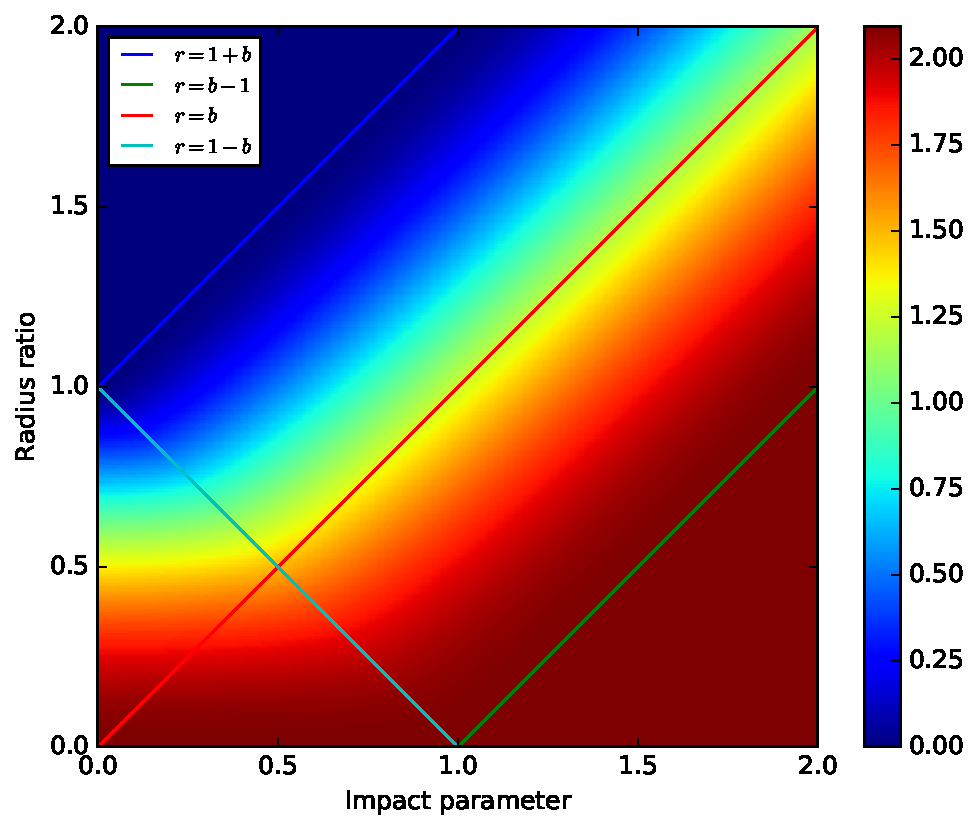
\includegraphics[width=0.85\linewidth]{figures/julia/transit_linear.pdf}
    \caption{The intensity of a linearly limb-darkened star ($u_1=1$) being
    eclipsed, $s_2(b,r)$.
    In the limit $b > r+1$, no eclipse occurs, so $s_2=1$.  For $b < r-1$, the star
    is completely eclipsed and $s_2=0$.  In the limits $b=r$ and $b=1-r$, special
    expressions must be used}
    \end{centering}
\end{figure}

\begin{figure}\label{s2_plot}
    \begin{centering}
    \includegraphics[width=0.85\linewidth]{figures/julia/s2_residuals.pdf}
    \caption{The numerical error in computing the flux of an eclipsed,  linearly
    limb-darkened star ($u_1=1$), $s_2(b,r)$.}
    \end{centering}
\end{figure}

\begin{figure}\label{s2_machine}
    \begin{centering}
    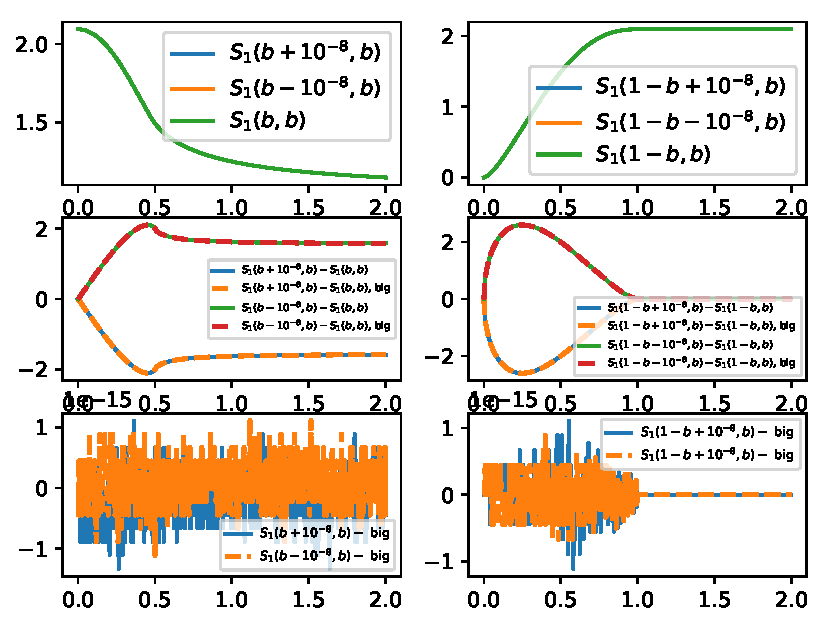
\includegraphics[width=\linewidth]{figures/julia/s2_machine.pdf}
    \caption{The accuracy of $s_2(b,r)$ near $b=r$ (left panel) and
    $b=1-r$ (right panel). The x-axese are impact parameter b,
    while the y axes in the top panels show $s_2(b,r)$, with $r$
    given in the legend of each panel. The middle panels plot
    the difference $(s_2(b,b\pm\epsilon)-s_2(b,b))/\epsilon$
    and $(s_2(b,1-b\pm\epsilon)-s_2(b,1-b))/\epsilon$. The bottom
    panels show the numerical precision by the comparing double precision
    computation with \texttt{BigFloat} precision (256-bit).}
    \end{centering}
\end{figure}


From \citet{MandelAgol2002}, the total flux visible during the occultation of a
body whose surface map is given by $I(\upmu)/I(1) = 1 - u_1(1 - \upmu)$ may be computed
as
\begin{eqnarray}
\frac{F(u_1,b,r)}{F_0} &=& \frac{u_1 s_2(b,r) + \pi(1-u_1)(1-\Lambda^e)}{\frac{2\pi}{3}u_1 + \pi(1-u_1)},\\
&=& 1-(1-u_1/3)^{-1}\left[(1-u_1)\Lambda^e(b,r) + u_1\left(\Lambda(b,r)+\tfrac{2}{3}\Theta(r-b)\right)\right],
\end{eqnarray}
where
\begin{align}
\Lambda^e(b,r) &=
\begin{dcases}
0 & \qquad 1+r \le b,\\
\frac{1}{\pi}\left[r^2 \cos^{-1}\left(\frac{1-r^2+b^2}{2b}\right) + \cos^{-1}\left(\frac{r^2+b^2-1}{2br}\right) \right.
                &\\ \phantom{XXXX}
\left.-\sqrt{\frac{4b^2-(1+b^2-r^2)^2}{4}}\right] & \qquad \vert 1-r\vert < b \le 1+r,\\
r^2 & \qquad b \le 1-r,\\
1 & \qquad b \le r-1,\\
\end{dcases}
\end{align}
and $F_0$ is the total unocculted flux.

% ==============================================================================
% ------------------------------------------------------------------------------
% ------------------------------------------------------------------------------
%
\clearpage
\section{Polynomial Limb-Darkening}
\label{sec:quad}
% ------------------------------------------------------------------------------
% ------------------------------------------------------------------------------
% ==============================================================================

In analogy with the linear and quadratic
limb-darkening laws, let us define the polynomial limb-darkening law of
order $l_\mathrm{max}$ as
%
%
\begin{align}
    \label{eq:polynomialld}
    \frac{I(\upmu)}{I(1)} &= 1 - u_1 (1 - \upmu) - u_2 (1 - \upmu)^2 - ... - u_{l_\mathrm{lmax}}(1 - \upmu)^{l_\mathrm{lmax}} \nonumber \\
                          &= \sum_{l=0}^{l_\mathrm{lmax}} \sum_{k=0}^l u_l {l \choose k} (-1)^k \upmu^k
    \quad,
\end{align}
%
where $u_0 \equiv 1$. For convenience, this can be expressed as the matrix equation
%
\begin{align}
    \label{eq:polynomialldmatrix}
    \frac{I(\upmu)}{I(1)} &= \bvec{u}^\top \, \bvec{L} \, \pmb{\upmu}
    \quad,
\end{align}
%
where $\bvec{u}^\top$ is a row vector whose value at index
$l$ is $u_l$, $\pmb{\upmu}$ is a column vector whose value at index $k$ is $\upmu^k$,
and $\bvec{L}$ is the lower triangular matrix with components given by
%
\begin{align}
    \label{eq:Llk}
    L_{lk} = {l \choose k} (-1)^k
    \quad.
\end{align}
%
It is straightforward to show that this law can be
expressed exactly as a sum over the $m = 0$ spherical harmonics, which also
form a complete basis of radially symmetric functions on the sphere.
%
Based on the relations in \citet{starry} for the spherical harmonics in Cartesian
form, the spherical harmonics of order $m = 0$ may be written
%
\begin{align}
    \label{eq:Ylzero}
    Y_{l,0}(\upmu) = \sqrt{\frac{2l + 1}{4\pi}}
              \sum_{k=0}^l {l \choose k} \frac{(k + l - 1)!!}{(k - l - 1)!!} \upmu^k
\end{align}
%
where $\upmu = z = \sqrt{1 - x^2 - y^2}$, $\binom{\bigdot}{\bigdot}$ is a binomial
coefficient, and $!!$ denotes the double factorial.

Our task now is to express the specific intensity function (\ref{eq:polynomialldmatrix})
in the basis of spherical harmonics (\ref{eq:Ylzero}). We therefore wish to find
the coefficients $c_l$ for which we may write
%
\begin{align}
    \label{eq:sphharmld}
    \frac{I(\upmu)}{I(1)} &= \sum_{l=0}^{l_\mathrm{lmax}} c_l Y_{l,0}(\upmu)
    \quad.
\end{align}
%
As before, we can write this as the matrix equation
%
\begin{align}
    \label{eq:sphharmldmatrix}
    \frac{I(\upmu)}{I(1)} &= \bvec{c}^\top \, \bvec{M} \, \pmb{\upmu}
    \quad,
\end{align}
%
where $\bvec{c}^\top$ is a row vector whose value at index
$l$ is $c_l$ and $\bvec{M}$ is the lower triangular matrix with components given by
%
\begin{align}
    \label{eq:Mlk}
    M_{lk} = \sqrt{\frac{2l + 1}{4\pi}} {l \choose k} \frac{(k + l - 1)!!}{(k - l - 1)!!}
    \quad.
\end{align}
%
Equating Equations~(\ref{eq:polynomialldmatrix}) and (\ref{eq:sphharmldmatrix}), we see
that we must have
%
\begin{align}
    \bvec{c}^\top \, \bvec{M} = \bvec{u}^\top \, \bvec{L} \quad,
\end{align}
%
or
%
\begin{align}
    \bvec{c} = (\bvec{M}^{-1} \, \bvec{L})^\top \bvec{u} \quad.
\end{align}
%
In \citet{starry} we described how to compute analytic transit and occultation light curves
for bodies whose surfaces are expressed as a sum over spherical harmonic coefficients. We
defined a body's surface map as the vector of spherical harmonic coefficients $\bvec{y}$.
The vector $\bvec{y}$ corresponding to our coefficients for the $Y_{l,0}$ harmonics is
related to $\bvec{c}$ via
%
\begin{align}
    y_{l(l + 1)} &= c_l
\end{align}
%
for $0 \leq l \leq l_\mathrm{max}$, where the values at all other indices in $\bvec{y}$ are zero.

\begin{figure}[t!]
    \begin{centering}
    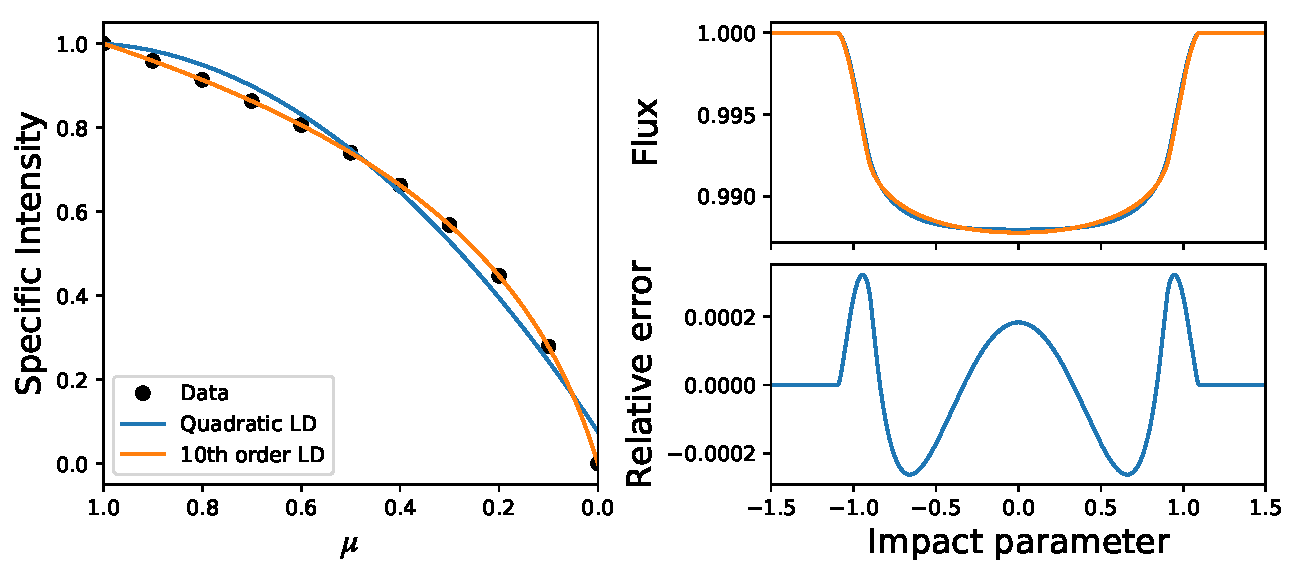
\includegraphics[width=\linewidth]{figures/python/high_order_ld.pdf}
    \caption{\label{fig:high_order_ld} Tenth order limb-darkening example with \starry. }
    \end{centering}
\end{figure}

{\color{red}We should derive simplified expressions of our formulae in \starry for the $m = 0$ case.} \todo{}

\begin{align}
    \label{eq:PGnI}
    \mathcal{P}(\bvec{G}_n) &=
    \begin{dcases}
        %
        r^{l+2} \sum\displaylimits_{i=0}^{\frac{l}{2}}
                {\frac{l}{2} \choose i}
                \left(\frac{b}{r}\right)^{\frac{l-2i}{2}}
                \mathcal{I}_{\frac{l+4}{2}, i}
            %
            & \qquad \frac{l}{2} \, \mathrm{even}
        \\[1em]
        %
        -r^{l-2} \left( b \mathcal{J}_{l-3,1} + r \mathcal{J}_{l-3,2} \right)
        %
        & \qquad l = 1
        \\[1em]
        %
        r^{l-1} \sum\displaylimits_{i=0}^{\frac{l-1}{2}}
                {\frac{l-1}{2} \choose i}
                \left(\frac{b}{r}\right)^{\frac{l-2i-1}{2}}
                \mathcal{J}_{\frac{l-1}{2}, i}
            & \qquad \frac{l-1}{2} \, \mathrm{even}
        \\[1em]
        %
        0 & \qquad \mathrm{otherwise}
    \end{dcases}
%
\end{align}
%
\begin{align}
%
    \nonumber \\
    \label{eq:QGnI}
    \mathcal{Q}(\bvec{G}_n) &=
    \begin{dcases}
        \mathcal{H}_{\frac{l+4}{2}, \frac{l}{2}}
        & \qquad \qquad \qquad \qquad \quad \quad \quad \quad \frac{l}{2} \, \mathrm{even}
        \\[1em]
        %
        0
        & \qquad \qquad \qquad \qquad \quad \quad \quad \quad \mathrm{otherwise} \quad.
    \end{dcases}
\end{align}

\bibliography{limbdark}

\end{document}
